\documentclass[a4paper,12pt]{article}
\usepackage{ucs}
\usepackage[utf8x]{inputenc}
\usepackage{amsfonts}
\usepackage[english,russian]{babel}
\usepackage[T1,T2A]{fontenc}
\frenchspacing
\usepackage{amsmath,amssymb,amsthm}
\usepackage[a4paper, margin=1in]{geometry}
\usepackage[table]{xcolor}
\usepackage{multirow}
\usepackage{diagbox}
\usepackage{graphicx}
\usepackage{listings}
\usepackage{minted}
\graphicspath{ {./} }

\newtheorem{name}{Printed output}
\newtheorem{problem}{Задача}
\newenvironment{solution}{\renewcommand{\proofname}{\unskip\indent\nopunct}\begin{proof}}{\end{proof}}

\begin{document}

\title{ДЗ 8}
\author{Витя\,Ефремов}
\maketitle

\begin{problem}
В приложенном файле дано распределение некоторого количества студентов по росту.
Построить гистограмму относительных частот (вручную или с использованием любых программ).
Найти несмещенные оценки для выборочного среднего, выборочной дисперсии.
Найти доверительный интервал для матожидания с уровнем надежности 0.9, 0.96, 0.98.
\end{problem}

\begin{solution}
Сделаем все с помощью  небольшого скрипта на питоне.


\inputminted{python}{hw_8.py}

\newpage
Оценка для выборочного среднего:
$$\bar{X} = 167.132$$
Оценка для выборочной дисперсии:
$$S^2 = 56.628$$
Доверительные интервалы для оценки матожадания с разными порогами:
\begin{table}[h!]
    \centering
    \begin{tabular}{|c|c|}
        \hline
        0.9  & $(154.755, 179.510)$ \\ \hline
        0.96 & $(151.678, 182.587)$ \\ \hline
        0.98 & $(149.626, 184.638)$ \\ \hline
    \end{tabular}
\end{table}

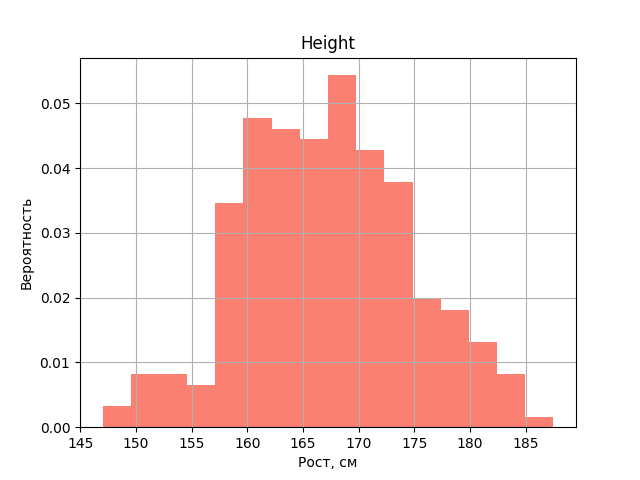
\includegraphics[width=\textwidth]{hist.png}

\end{solution}
\end{document}
